\chapter{Groupe Work}

\section{Case Exercises}

\subsection{Case 1 (Intro Case; Parma Ham A/S) - 03.09.24}


\subsubsection*{Information}
\begin{highlight}
    The information given for this case is as follows:

\begin{itemize}
\item Production capacity: 330.000 raw hams per year
\item 70 well-educated staff members
\item Production of Parma ham
\item Has experienced huge problems with Salmonella and
\item Staphylococcus aureus during the production of Parma ham
\item Therefore, Parma Ham A/S has obtained an ISO 22000
certification

\end{itemize}
\end{highlight}


\subsubsection*{Company Policy}
\begin{highlight}
    The information given for this case is as follows:

\begin{itemize}
\item Parma Ham A/S will produce high quality Parma ham safe for human consumption.
\item The Food Safety Management System (FSMS), complying with the requirements given in “DS/EN ISO22000:2018”, shall ensure that legal requirements as to food safety are fulfilled at any time.
\item The FSMS shall ensure that customer requirements as to food safety are fulfilled at any time.
\item The presence of Salmonella and Staphylococcus aureus shall be reduced to an acceptable level at Parma Ham A/S.
\item All staff members at Parma Ham A/S shall be aware of the food safety policy and the FSMS.

\end{itemize}
\end{highlight}


\subsubsection{\textit{Salmonella ssp.}}
\begin{highlight}
    The information given for this case is as follows:

\begin{itemize}
\item Pathogenic Gram negative bacterium
\item Naturally found in the intestinal tracts of mammals, birds, amphibians and reptiles but not in fish crustaceans or mollusks
\item Causing salmonellosis
\subitem Nausea, vomiting, abdominal cramps and fever 
\subitem Zoonotic infection
\item The infective dose of Salmonella is thought to be extremely variable, relatively high for healthy individuals and very low for at-risk individuals, such as the elderly or medically compromised.
\item Facultative anaerobe
\item Minimum water activity for growth is 0.94
\subitem (~ max. 8\% salt in water phase)
\item Able to survive in dried foods
\item Min(/max) temperature for growth is 5 (46)\textdegree C
\item Min(/max) pH for growth is 3.7 (9.5)
\item The presence of Salmonella can be prevented by: heating food sufficiently to kill the bacteria, holding chilled food below 5\textdegree C, preventing post-cooking cross-contamination and prohibiting people who are ill or are carriers of Salmonella from working in food operations

\end{itemize}
\end{highlight}


\subsubsection{\textit{Staphylococcus aureus}}
\begin{highlight}
    The information given for this case is as follows:

\begin{itemize}
\item Pathogenic Gram positive bacterium
\item Humans and animals are the primary reservoirs for Staph. aureus. Staph. aureus can be found in the nose and throat and on the hair and skin of 50 percent of healthy individuals. However, the bacteria can be found in air, dust, sewage and surfaces of food-processing equipment. Staph. aureus can produce a toxin if allowed to grow in food. The toxin is not destroyed by the cooking or canning processes
\item Staph. aureus food poisoning causes nausea, vomiting,
abdominal cramping, watery or bloody diarrhea, and fever
\item Facultative anaerobe
\item Min(/max) temperature for growth is 7 (50)\textdegree C
\item Min(/max) pH for growth is 4 (10)
\item S. aureus has the ability to grow and produce toxins in food with very little available water (aw 0.86, 20 percent salt in water phase), which would prevent the growth of other pathogens.
\item The presence of Staph. aureus can be prevented by:
minimizing time/temperature abuse of food, especially after
cooking, and requiring that food handlers engage in proper
hygiene.

\end{itemize}
\end{highlight}

\newpage

\subsubsection*{Organizational Structure}
\begin{figure}[h]
    \centering
    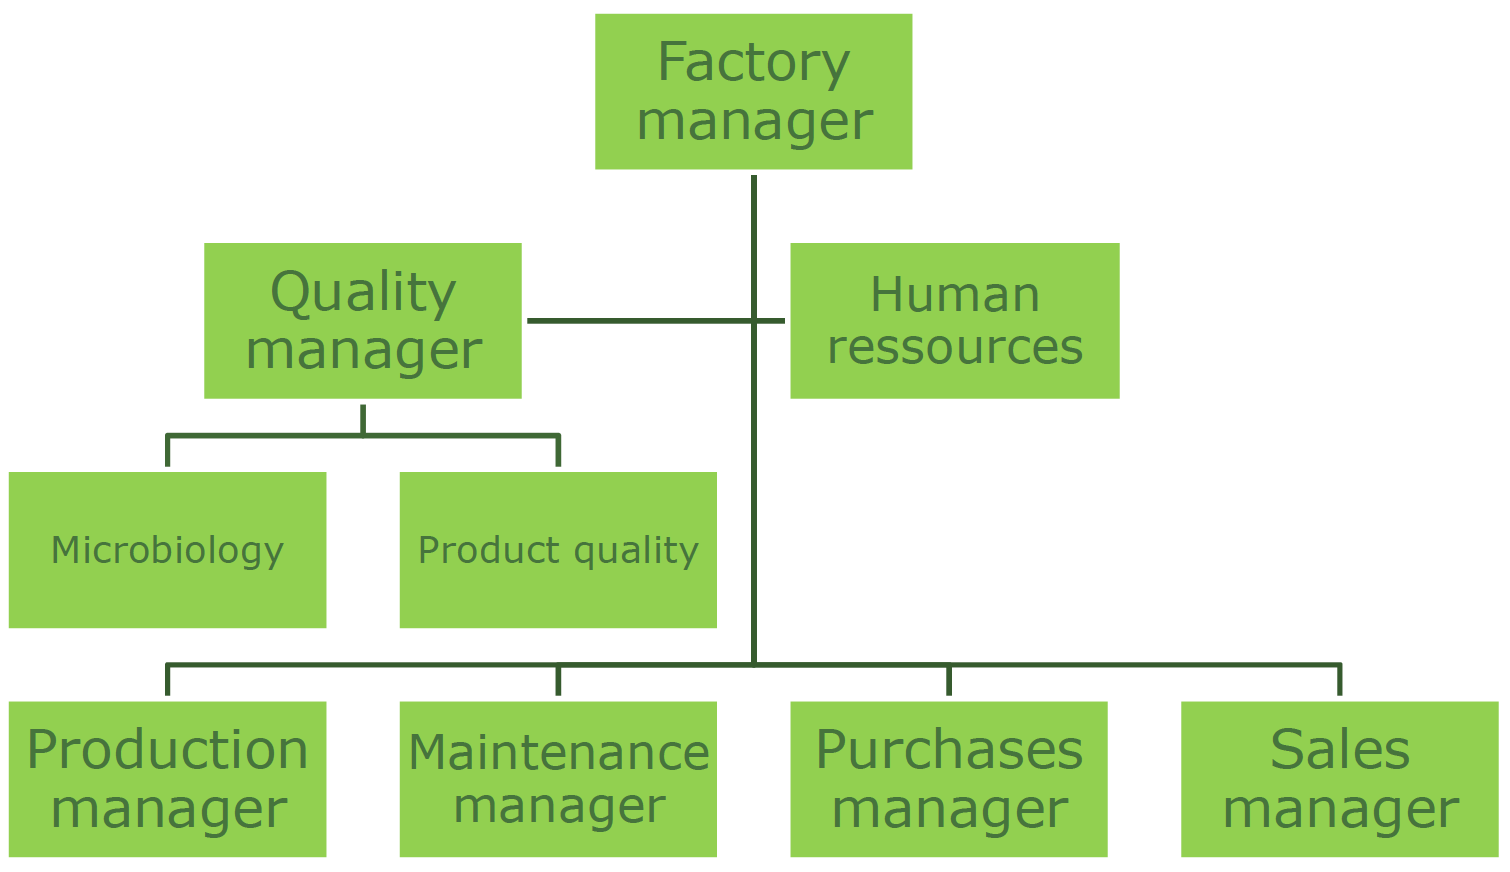
\includegraphics[width=0.8\textwidth]{Figures/Parma Ham - Organization Diagram.png}
    \caption{Organizational structure of Parma Ham A/S}
    \label{fig:ParmaHamAS}
\end{figure}

\subsubsection*{Responsibilities}
 
\begin{highlight}
    The information given for the organizational structure and roles is as follows:

\begin{itemize}
\item The Factory Manager is responsible for:
\subitem - The overall management of the factory, including the implementation of 
\subitem - The FSMS.
\subitem - Shall ensure adequate ressources for development and implementation of the Food Safety \subitem Management System and for continually improving its effectiveness

\item The Quality Manager is the overall responsible for:
\subitem - The Food Safety Management System
\subsubitem * Development
\subsubitem * Implementation
\subsubitem * Maintenance

\item The Production Manager is responsible for:
\subitem  - The production of the Parma ham and for inspection of raw materials
\subitem - The production staff is divided into
several sections, each with a section leaders
\subitem - The section leaders are responsible for
\subitem - Ensuring that all staff members have the necessary competencies
\subitem - Ensuring that all staff members
have the necessary food safety awareness
\subitem - Education and training of staff members

\end{itemize}
\end{highlight}

\begin{highlight}
    Information continued:
    \begin{itemize}
        \item The Sales Manager is responsible for:
        \subitem - Customer focus
        \subitem - Investigating the requirements and expectations of customers
        \subitem - Investigating whether these requirements and expectations are fulfilled

        \item The Purchasing Manager is responsible for:
        \subitem - Supplier focus
        \subitem - Ensuring that purchased products conform to specified purchase requirements
        \subitem - Specified purchase requirements
        \subsubitem * Approval of products, procedures, processes and equipment
        \subsubitem * Qualification of personnel
        \subsubitem * QMS/FSMS
        \subitem - Supplier audits

    \end{itemize}
\end{highlight}


\subsection{Easy Case 1 - 10.09.24}
In this easy case, we are tasked to sit 30 minutes by ourselves and write down the answers to the following questions. After the 30 minutes, we will discuss the answers in our designated groups and prepare a presentation for 15 minutes. One group will be assigned to hold a presentation of the easy case. The following background and tasks has been given to us.

\subsubsection*{Background}
You are a food safety manager at a mid-sized food processing company. Your company specializes in producing juice products, and maintaining high standards of food safety and quality is paramount. Recently, your company decided to implement ISO 22000:2018 to enhance its food safety management system and improve process control. As part of this initiative, you are tasked with developing a comprehensive monitoring procedure targeting biological and physical hazards, as well as integrating Statistical Process Control (SPC) methods to manage variability in the production process.

\subsubsection*{Task}
The following bulletpoints are the tasks that you need to address in this case:
\begin{itemize}
    \item Define three natural and three assignable variations in the context of SPC and juice production and their relevance to food safety management.
    \item Identify three control measures targeting biological (\textit{Salmonella}) or physical (glass pieces) hazards in juice production.
    \item Provide examples of sensors or measurement techniques that can be used to monitor these control measures to ensure they are effective.
\end{itemize}

\subsubsection*{Personal Notes}

\textbf{Bulletpoints from the background:}
\begin{itemize}
    \item Product = juice
    \item Implementing ISO 22000:2018
    \item Monitoring procedure targeting biological and physical hazards
    \item Integrating Statistical Process Control (SPC) methods
\end{itemize}

\vspace{2\baselineskip}

\textbf{Answers to the task:}
\vspace{1\baselineskip}

Three natural variations which can affect the production of juice and food safety management:
\begin{itemize}
    \item Seasonal variations in the raw materials which can affect the quality of the juice and the growth of pathogens
    \item Variations in the temperature of the production environment which can affect the growth of pathogens
    \item Variations in the pH of the juice which can affect the growth of pathogens or the stability of the product
\end{itemize}

\vspace{1\baselineskip}

Three assignable variations which can affect the production of juice and food safety management:
\begin{itemize}
    \item Equipment malfunction in the production line
    \item Human error in the production process
    \item Contamination of raw materials or final product
\end{itemize}

\vspace{1\baselineskip}

Three control measures which can be implemented to target biological or physical hazards in juice production:
\begin{itemize}
    \item Heat treatment of the juice to kill pathogens which can cause foodborne illnesses e.g. \textit{Salmonella}
    \item Filtration of the juice to prevent glass pieces from entering the final product
    \item Cleaning and sanitation of the production environment for overall good manufacturing practices
\end{itemize}

\vspace{1\baselineskip}

Examples of sensors or measurement techniques that can be used to monitor these control measures:
\begin{itemize}
    \item Temperature sensors to monitor the heat treatment process of the juice. Thus ensuring that the pathogens are killed
    \item pH meters to monitor the pH of the juice. Thus ensuring that the product is stable and safe for consumption. Also in-line pH sensors can be used to monitor the pH continuously
    \item Random sampling of the incoming raw products to ensure the composition and quality of the raw materials. 
    \item Testing of equipment to ensure that they are functioning properly and not contaminating the final product or leaving glass pieces in the juice
    \item Training employees to ensure that they are following good manufacturing practices and are trained in operating the equipment properly
    \item Perform tritration on cleaning detergent to ensure that the cleaning is effective and that the equipment is sanitized properly
    \item In-line X-Ray screening of the product to ensure that there are no glass pieces in the the product
\end{itemize}


